\section{Introduction}
When studying intelligence, insects, reptiles, and humans have been found to possess neurons with the capacity to hold integers, real numbers, and perform arithmetic operations \cite{nieder-neuronal-number,rugani-arithmetic-chicks,gallistel-numbers-in-brain}.
In our quest to mimic intelligence we have put much faith in neural networks, which in turn has provided unparalleled and often superhuman performance in tasks requiring high cognitive abilities \cite{natureGo,bert,openai-learning-dexterous}.
However, when using neural networks to learn simple arithmetic problems, such as counting, multiplication, or comparison they systematically fail to extrapolate onto unseen ranges \cite{stillNotSystematic,suzgun2019evaluating,trask-nalu}. This can be a significant drawback when comparing in question answering \cite{naturalquestions} or counting objects in visual data \cite{johnson2017clevr,drewspaper}.

In this paper, we analyze and improve parts of the recently proposed Neural Arithmetic Logic Unit (NALU) \cite{trask-nalu}.
The NALU is a neural network layer with two sub-units; the $\text{NAC}_{+}$ for addition/subtraction and the $\text{NAC}_{\bullet}$ for multiplication/division.
The sub-units are softly gated using a sigmoid function. The parameters, which are computed by a soft weight constraint using a tanh-sigmoid transformation, are learned by observing arithmetic input-output pairs and using backpropagation \cite{rumelhart1986learning}.

Our contributions are alternatives to the $\text{NAC}_{+}$ and $\text{NAC}_{\bullet}$ units that are more theoretically founded. Our alternatives can support small and negative numbers, are more sparse, and supports a larger hidden size, while using less parameters.
We test these properties through a rigid experimental setup with more than 10000 arithmetic tests and recurrent multiplication of up to 20 MNIST digits \cite{mnist}.
%More specifically;
%an alternative formulation of the soft weight constraint with a clipped linear activation, parameter regularization that biases towards a sparse solution of $\{-1,0,1\}$, and a reformulation of the multiplication unit with a partial linearity. All of which significantly improves upon the $\text{NAC}_{+}$ and $\text{NAC}_{\bullet}$ units as shown through extensive testing on static arithmetic tasks (more than $10000$ experiments) and recurrent multiplication of a sequence of MNIST digits.

\begin{figure}[h]
\centering
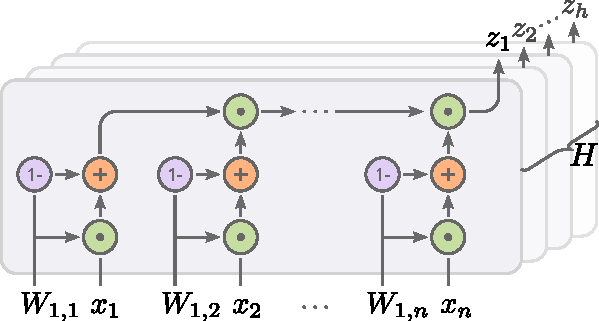
\includegraphics[scale=0.6]{graphics/nmu.pdf}
\caption{Visualization of NMU for a single output scalar $z_1$, this construction repeats for every element in the output vector $\mathbf{z}$.}
\end{figure}
We motivate our work by an investigation of the NALU components: the soft gating mechanism that binds the subunits; the subunits $\text{NAC}_{\bullet}$ and $\text{NAC}_{+}$, and the way parameters are constructed.
Our findings are the following:
(a) $\text{NAC}_{\bullet}$ does not work for negative input.
(b) $\text{NAC}_{\bullet}$ cannot model inputs $<\epsilon$.
(c) optimal weight initialization for the parameters has a gradient of zero in expectation.
(d) the weight design does not enforce sparsity and results suggests that they rarely are, which limits interpretability.
(e) $\text{NAC}_{\bullet}$ has no optimal initialization.
(f) The expected mean of $\text{NAC}_{\bullet}$, at initialization, is exponential w.r.t. the hidden size and has exploding variance.
(g) Optimizing $\text{NAC}_{\bullet}$ for division is close to impossible and never converges in practice.
(h) The NALU does not converge; we find that learning the gate is cumbersome due to the heterogeneity of the subunits. $\text{NAC}_{\bullet}$ takes orders of magnitude longer to converge than $\text{NAC}_{+}$.%, and their estimated gradient signals has varying magnitude.

Motivated by these challenges, we attempt to solve (a-f) and leave (g-h) for future work.

Furthermore, we find that the experimental setup of \citet{trask-nalu} has the following concerns: (i) the dataset parameters for "simple function task" is not defined. (ii) the evaluation metric is based on relative performance to a random baseline. This means that if the random baseline has an MSE of 1e10, then 1e7 would be considered a score of 0.1. (iii) Multiplication is only thoroughly tested in simple function task and not on anything requiring a deep neural network \todo{(comments on 4.3 in appendix XX)}.

We attempt to solve (i-iii) by proposing a much extended arithmetic task, define a successful convergence criteria, and do multiplication of MNIST digits.
% The investigation uncovers the following analytical and empirical concerns; the gradients of the weight matrix construction in $\text{NAC}_{+}$ and $\text{NAC}_{\bullet}$ have zero expectation, the $\text{NAC}_{\bullet}$ has a treacherous optimization space with unwanted global minimas near singularities, when applying the $\text{NAC}_{+}$ in isolation we observe that the wanted weight matrix values of $\{-1, 0, 1\}$ are rarely found, and our empirical results reveals that the NALU is significantly worse than hard-choosing either the $\text{NAC}_{+}$ or $\text{NAC}_{\bullet}$, indicating that the gating mechanism does not work as intended.

% We avoid using gating as we see no obvious solution to simultaneously train two vastly different sub-units, the NAU/$\text{NAC}_{+}$ and NMU/$\text{NAC}_{\bullet}$, with a soft gating mechanism. We expand upon why this is such a big challenge in section \ref{sec:methods:gatting-issue} and show empirically in \ref{} that this gating .
% We will thus assume that the desired operation is already known, or can empirically be found by varying the network architecture.

\subsection{Learning a 10 parameter function}
Consider the static function $t = (x_1 + x_2) \cdot (x_1 + x_2 + x_3 + x_4)$ for $x \in \mathbb{R}^4$. To illustrate the ability of $\mathrm{NAC}_{\bullet}$, NALU, and our proposed NMU, we conduct 100 experiemnts for each mode, where we attempt to fit this function. Table \ref{tab:very-simple-function-results} show that NMU has a higher success rate and converges faster.
%When inspecting the $6\%$ that did not converge, we found the issue to be underflow when $w = 0$ in the multiplication layer.
\begin{table}[!h]

\caption{\label{tab:very-simple-function-results}Shows the success-rate, at what global step the model converged at, and the sparsity error for all weight matrices, with 95\% confidence interval. Best result is highlighed.}
\centering
\begin{tabular}{crllll}
\toprule
\multicolumn{1}{c}{Op} & \multicolumn{1}{c}{Model} & \multicolumn{1}{c}{Success} & \multicolumn{2}{c}{Solved at} & \multicolumn{1}{c}{Sparsity error} \\
\cmidrule(l{3pt}r{3pt}){1-1} \cmidrule(l{3pt}r{3pt}){2-2} \cmidrule(l{3pt}r{3pt}){3-3} \cmidrule(l{3pt}r{3pt}){4-5} \cmidrule(l{3pt}r{3pt}){6-6}
 &  & Rate & Median & Mean & Mean\\
\midrule
 & $\mathrm{NAC}_{\bullet}$ & $13\% {~}^{+8\%}_{-5\%}$ & $5.5 \cdot 10^{4}$ & $5.9 \cdot 10^{4} {~}^{+7.8 \cdot 10^{3}}_{-6.6 \cdot 10^{3}}$ & $7.5 \cdot 10^{-6} {~}^{+2.0 \cdot 10^{-6}}_{-2.0 \cdot 10^{-6}}$\\

 & NALU & $26\% {~}^{+9\%}_{-8\%}$ & $7.0 \cdot 10^{4}$ & $7.8 \cdot 10^{4} {~}^{+6.2 \cdot 10^{3}}_{-8.6 \cdot 10^{3}}$ & $9.2 \cdot 10^{-6} {~}^{+1.7 \cdot 10^{-6}}_{-1.7 \cdot 10^{-6}}$\\

\multirow{-3}{*}{\centering\arraybackslash $\bm{\times}$} & NMU & $\mathbf{94\%} {~}^{+3\%}_{-6\%}$ & $\mathbf{1.4 \cdot 10^{4}}$ & $\mathbf{1.4 \cdot 10^{4}} {~}^{+2.2 \cdot 10^{2}}_{-2.1 \cdot 10^{2}}$ & $\mathbf{2.6 \cdot 10^{-8}} {~}^{+6.4 \cdot 10^{-9}}_{-6.4 \cdot 10^{-9}}$\\
\bottomrule
\end{tabular}
\end{table}

